\subsection{Comunicación entre plataformas}\label{ssection:comunicacion_plataformas}
La conexión entre la parte de los vehículos a motor y de los ciclistas hacia la nube
se establece a través de tecnología móvil \gls{lte} o \gls{3g}, dependiendo de la
disponibilidad, aunque la manera de comunicarse con la \emph{Nube de Conductores} es
diferente. La Nube de Conductores actúa como intermediario entre las aplicaciones
desarrolladas en el lado de los motoristas (Sección \ref{section:comunicacion_vehicular})
y el de los ciclistas (Sección \ref{section:appCiclistas}).

\subsubsection{Mensajes a ciclistas}\label{sssection:mensajes_ciclistas}
Gracias al actual predominio de Smartphones en la vida de todos los habitantes, el
despliegue de aplicaciones móviles vehiculares es bastante sencillo. Se han convertido
en dispositivos potentes y versátiles, los cuales permiten utilizarlos para una gran
variedad de utilidades. Gracias que tienen GPS integrado podemos obtener una posición
bastante aproximada de los usuarios, dependiendo de la calidad del dispositivo se obtendrá
una localización más precisa. También poseen conexión móvil con una gran variedad
de conexiones como Bluetooth, USB, Wi-Fi, LTE, GSM, UMTS y NFC.

Actualmente el predomino del mercado se encuentra en el Sistema Operativo móvil Android.
Este sistema, actualmente en desarrollo por Alphabet, esta orientado principalmente a
dispositivos móviles y embebidos. Esta basado en Linux, y es un proyecto que tiene
devoción por los estándares abiertos existentes; prueba de ello es la pertenencia a
la alianza comercial Open Handset Alliance, la cual se dedica a desarrollar estándares
abiertos para su uso en dispositivos móviles.

Android posee un completo entorno de desarrollo, el cual incluye un depurador de
código, biblioteca, un simulador de teléfono, documentación, ejemplos de código y
tutoriales. Para el desarrollo en esta plataforma se puede optar por dos opciones, la
instalación del IDE de desarrollo Android Studio, ó descargar el SDK de Android e
integrarlo con el IDE que se desee. Los lenguajes de programación con los que es
posible desarrollar son Java y C/C++, aunque este segundo solo se recomienda su uso
para el desarrollo de librerías que requieran de un gran rendimiento. La aplicación
resultante es un paquete apk que es ejecutado en un Sandbox dentro de Android.

Se ha desarrollado una aplicación \emph{Android} desde la cual se manda a la nube
actualizaciones sobre la posición del usuario o el grupo que el usuario haya creado.
\'Este recibe notificaciones sobre las posiciones de los vehículos próximos, y otros
diferentes eventos que pueden darse en la carretera; por ejemplo, un accidente de
tráfico. Se ha contemplado la posibilidad de salidas en grupo de ciclistas, para ello
se ha habilitado una modalidad específica mediante la cual se crea un grupo que se
comunica entre sus miembros a través de una red privada \emph{Wi-Fi 802.11}. Los
diferentes miembros se mantienen actualizados sobre los diferentes eventos a través
de un nodo denominado líder, el cual es el enlace a la nube tanto para reportar la
posición del grupo de ciclistas como para recibir mensajes de la nube y retransmitir
éstos al resto de miembros.

Para comunicarse con los dispositivos Android se requiere un sistema de comunicación
por el cual aunque los ciclistas no tengan en un momento determinado cobertura, los
mensajes no se pierdan. Se ha elegido la plataforma \gls{gcm}, la cual se encarga de
gestionar que los mensajes lleguen al destino aunque éste se encuentre temporalmente
inaccesible mediante tecnología \emph{Push} [\ref{alg:gcmFuncionamientoMensajes}].

El mensaje debe respetar el formato que la API de GCM indica y puede observarse en
el algoritmo \ref{alg:gcmformato}, donde \emph{ID\_ANDROID} es el identificador del
dispositivo Android al que se le va a enviar el mensaje, y \emph{DATOS} un objeto
\emph{JSON} con la información se que desea enviar. Para crear un identificador único,
se puede emplear el que crea Android cuando se introduce la cuenta de correo personal
en el móvil. Un identificador de Android está formada por una cadena hexadecimal de
64 bit, la cual es poco probable que se repita. En el caso de que se quisiese reducir
aún más la probabilidad de repetición, se puede mezclar el identificador de Android
con el que la compañía de telefonía emplea para identificar nuestro dispositivo; aunque
esto último aumenta el tamaño de los mensajes.

\begin{listing}
	\begin{minipage}{.4\textwidth}
		\begin{minted}[linenos=true]{java}
{ "registration_ids": [ "ID_ANDROID" ], data: { /*DATOS*/ }}
		\end{minted}
	\end{minipage}
	\caption{Envío de mensajes mediante GCM}\label{alg:gcmformato}
\end{listing}

% FALTA EXPLICAR
\begin{figure}[H]
	\begin{center}
		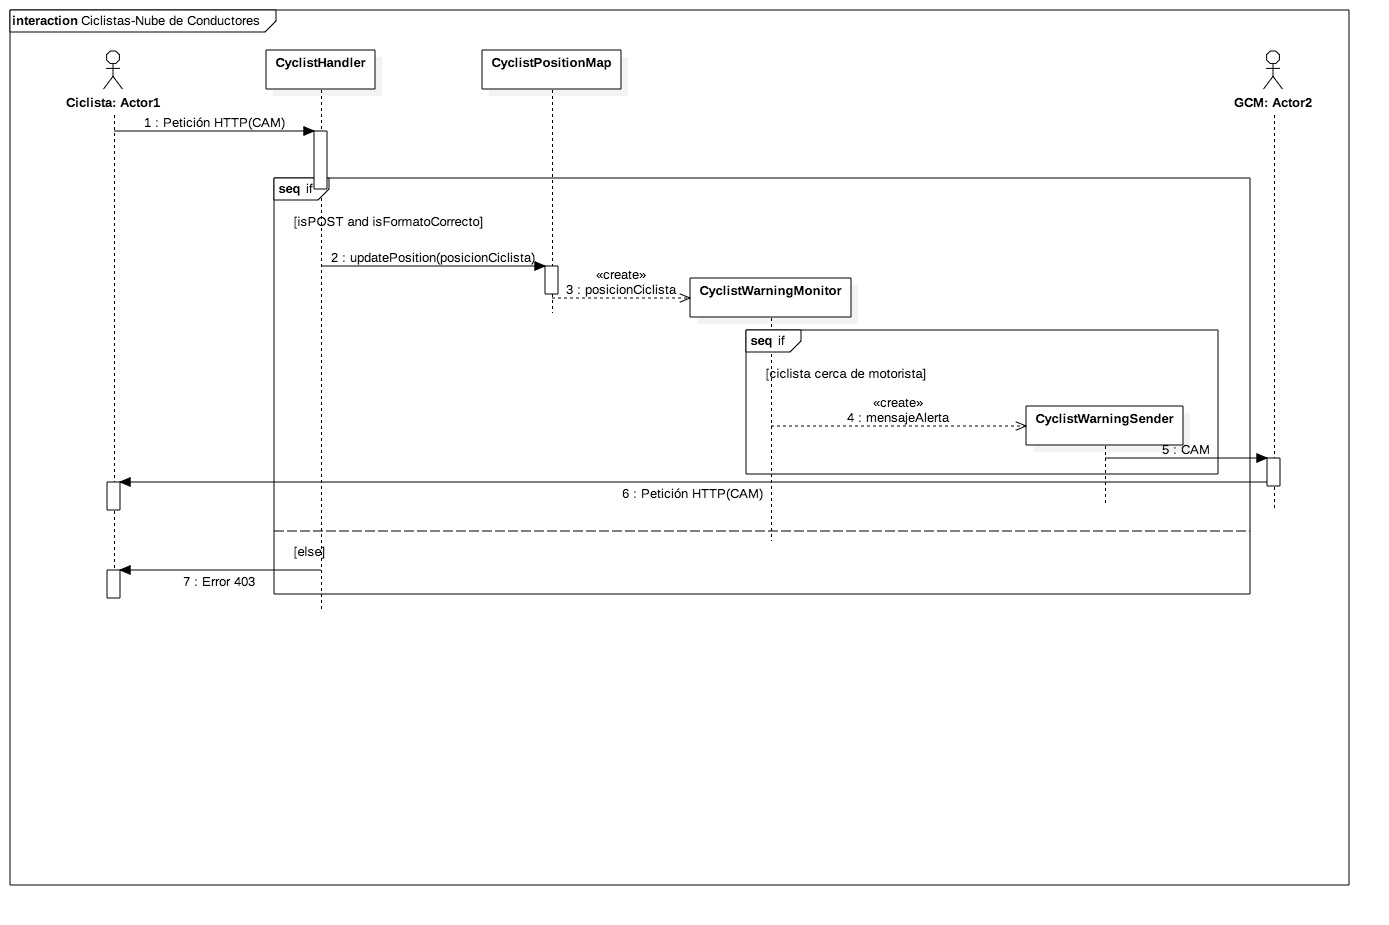
\includegraphics[scale=0.4]{DiagSecuencia-Ciclistas_Cloud}
		\caption{Ejecución entre Ciclista y la Nube}
		\label{fig:DiagSecuencia-OBU_Cloud}
	\end{center}
\end{figure}

\subsubsection{Mensajes a vehículos a motor}\label{sssection:mensajesvehiculomotor}
Los vehículos poseen un dispositivo \gls{obu} que permite comunicarse con la infraestructura
en carretera a través de una red \emph{IEEE 802.11p}. Gracias a las \gls{rsu} dispuestas
en la carretera, las cuales actúan de intermediario, se envían y reciben los mensajes
de la nube. Esto es posible gracias a la implementación de servlets que escuchan mensajes
provenientes por el puerto 8080. Por tanto puede decirse, que las \gls{rsu} actúan de
\emph{gateway} de comunicaciones entre los vehículos y las aplicaciones desplegadas
en la \emph{Nube de Conductores}. La \gls{obu} al recibir el mensaje lo muestra en
un Interfaz Humano-Máquina (\emph{HMI}) que posee el vehículo. La información del vehículo
puede ser recogida a través de un interfaz \emph{OpenXC} ó/y la \gls{obu}, dependiendo
de la tecnología que se emplee para ello.

Los mensajes enviados a los vehículos a motor siguen el formato mostrado en la sección
\ref{ssection:FormatoMensajesNC}. La \emph{Nube de Conductores} envía mensajes HTTP/1.1
a través del método POST un mensaje con contenido JSON a la \gls{rsu}. Ésta se encarga
de reenviarlo al vehículo a través de la red \emph{IEEE 802.11p}.

\begin{figure}[H]
	\begin{center}
		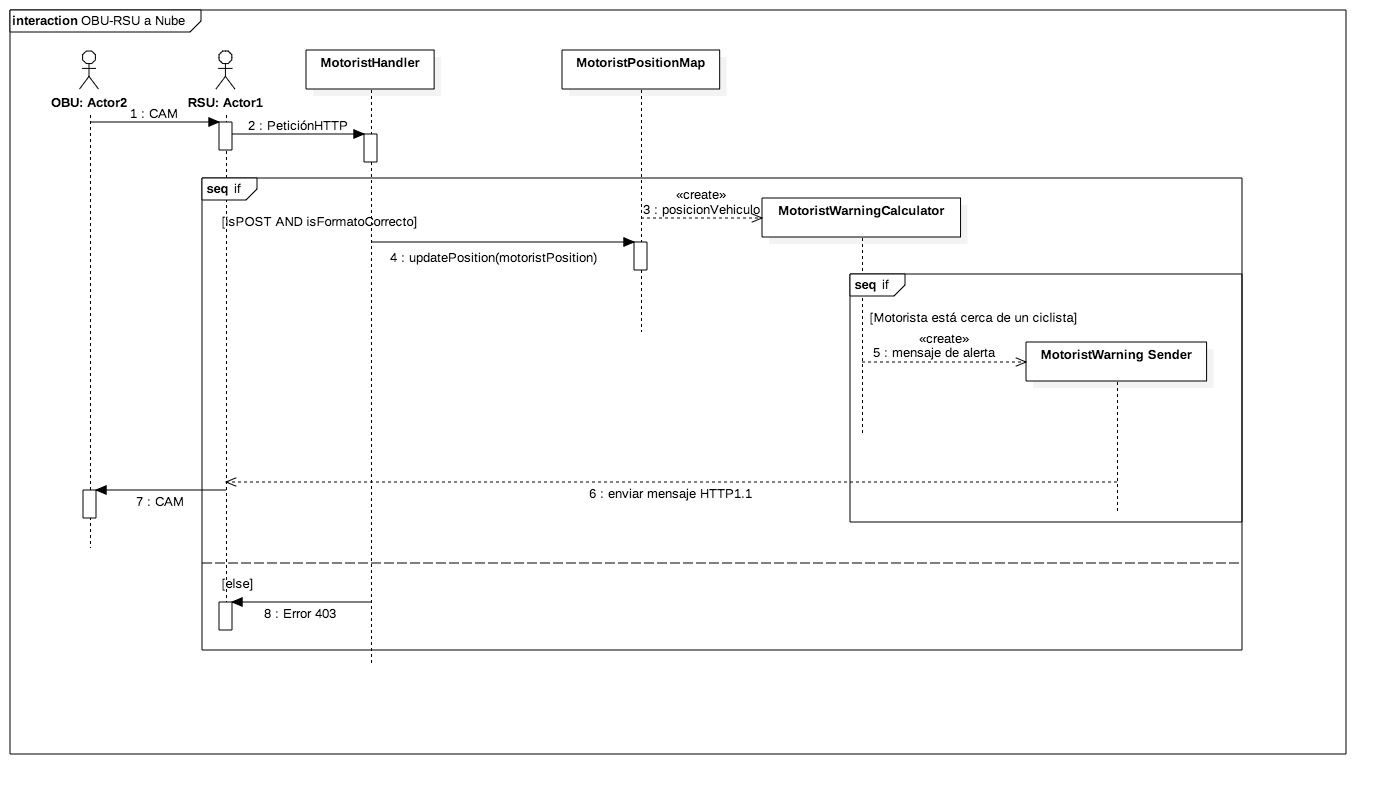
\includegraphics[scale=0.4]{DiagSecuencia-OBU_Cloud}
		\caption{Ejecución entre OBU, RSU y la Nube}
		\label{fig:DiagSecuencia-OBU_Cloud}
	\end{center}
\end{figure}

